\let\negmedspace\undefined
\let\negthickspace\undefined
\documentclass[journal,12pt,onecolumn]{IEEEtran}
\usepackage{cite}
\usepackage{amsmath,amssymb,amsfonts,amsthm}
\usepackage{algorithmic}
\usepackage{graphicx}
\graphicspath{{./figs/}}
\usepackage{textcomp}
\usepackage{xcolor}
\usepackage{txfonts}
\usepackage{listings}
\usepackage{enumitem}
\usepackage{mathtools}
\usepackage{gensymb}
\usepackage{comment}
\usepackage{caption}
\usepackage[breaklinks=true]{hyperref}
\usepackage{tkz-euclide} 
\usepackage{listings}
\usepackage{gvv}                                        
%\def\inputGnumericTable{}                                 
\usepackage[latin1]{inputenc}     
\usepackage{xparse}
\usepackage{color}                                            
\usepackage{array}                                            
\usepackage{longtable}                                       
\usepackage{calc}                                             
\usepackage{multirow}
\usepackage{multicol}
\usepackage{hhline}                                           
\usepackage{ifthen}                                           
\usepackage{lscape}
\usepackage{tabularx}
\usepackage{array}
\usepackage{float}
%\newtheorem{theorem}{Theorem}[section]
%\newtheorem{theorem}{Theorem}[section]
%\newtheorem{problem}{Problem}
%\newtheorem{proposition}{Proposition}[section]
%\newtheorem{lemma}{Lemma}[section]
%\newtheorem{corollary}[theorem]{Corollary}
%\newtheorem{example}{Example}[section]
%\newtheorem{definition}[problem]{Definition}

\begin{document}

\title{4.6.8}
\author{EE25BTECH11018 - Darisy Sreetej}
% \maketitle
% \newpage
% \bigskip
%\begin{document}
{\let\newpage\relax\maketitle}
%\renewcommand{\thefigure}{\theenumi}
%\renewcommand{\thetable}{\theenumi}
\textbf{Question:}\\
Find the equation of the plane passing through the points having position vectors $\hat{i}+\hat{j}-2\hat{k},2\hat{i}-\hat{j}+\hat{k},\hat{i}+2\hat{j}+\hat{k}$.Write the equation of the plane passing through a point $(2, 3, 7)$ and parallel to the plane obtained above. Hence, find the distance between the two parallel planes. \\
\solution
\begin{table}[H]
	\centering
	\caption{}
	\begin{tabular}{|c|c|}
\hline
\textbf{Variable} & \textbf{Value} \\
\hline
$A$ & $(0,-\frac{3}{2})$ \\
\hline
$m$ & $\frac{1}{2}$ \\
\hline
\end{tabular}
	\label{}
\end{table}
Let the equation of plane be
\begin{align}
	\vec{n}^\top\vec{x}=C_1
\end{align}
A,B,C satisfies this equation,
\begin{align}
	\vec{n}^\top\vec{A}=C_1,
	\vec{n}^\top\vec{B}=C_1,
	\vec{n}^\top\vec{C}=C_1
\end{align}
\begin{align}
	\myvec{\vec{A}\\\vec{B}\\\vec{C}}^\top\vec{n}=\myvec{C_1\\C_1\\C_1}
\end{align}
Using augmented matrix,
\begin{align}
	\augvec{3}{1}{1&1&-2&C_1\\2&-1&1&C_1\\1&2&1&C_1}
\end{align}
$R_2=R_2-2R_1$\\
$R_3=R_3-R_1$
\begin{align}
	\augvec{3}{1}{1&1&-2&C_1\\0&-3&5&-C_1\\0&1&3&0}
\end{align}
$R_2 \Longleftrightarrow R_3$
\begin{align}
	\augvec{3}{1}{1&1&-2&C_1\\0&1&3&0\\0&-3&5&-C_1}
\end{align}
$R_3=R_3+3R_2$
\begin{align}
	\augvec{3}{1}{1&1&-2&C_1\\0&1&3&0\\0&0&14&-C_1}
\end{align}
\begin{align}
	14z+C_1=0\implies z=\frac{-C_1}{14} 
\end{align}
\begin{align}
	y+3z=0\implies y=\frac{3C_1}{14}
\end{align}
\begin{align}
	x+y-2z=C_1\implies x=\frac{9C_1}{17}
\end{align}
Let $C_1=14$
\begin{align}
	\vec{n}=\myvec{9\\3\\-1},C_1=14
\end{align}
Equation of the plane 
\begin{align}
    \myvec{9\\3\\-1}^\top\vec{x}=14
\end{align}
For finding parallel plane passing through P ,
\begin{align}
	\vec{n}^\top\vec{x}=C_2
\end{align}
\begin{align}
	\vec{n}^\top\vec{P}=C_2
\end{align}
\begin{align}
	C_2=\myvec{9&3&-1}\myvec{2\\3\\7}
\end{align}
\begin{align}
	C_2=20
\end{align}
Equation of plane parallel to given plane passing through point P is
\begin{align}
	\myvec{9\\3\\-1}^\top\vec{x}=20
\end{align}
The $2$ planes obtained are parallel since their normal vectors are the same\\
The normal vector of the planes $\vec{n}$
\begin{align}
\vec{n} = \myvec{9 \\ 3 \\ -1}
\end{align}

The distance between the planes is given by this formula
\begin{align}
\text{Distance} = \frac{\abs{d_1 - d_2}}{\norm{\vec{n}}}
\end{align}

Where $d_1 = 14$ and $d_2 = 20$

\begin{align}
{\norm{\vec{n}}} = \brak{\sqrt{\brak{9}^2 + \brak{3}^2 + \brak{-1}^2}} = \sqrt{91}
\end{align}
Substituting these values in the distance formula, we get
\begin{align}
\therefore \text{Distance} = \frac{\abs{14-20}}{\sqrt{91}}
\end{align}

\begin{align}
\text{Distance} = \frac{6}{\sqrt{91}}
\end{align}
\\
Therefore, the distance between the planes is $\frac{6}{\sqrt{91}}$
\begin{figure}[h!]
    \centering
    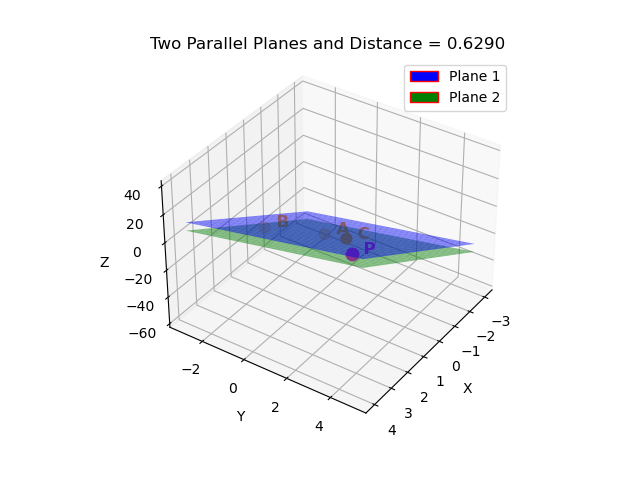
\includegraphics[height=0.5\textheight, keepaspectratio]{figs/fig.png}
    \label{figure_1}
\end{figure}
\end{document}

